\documentclass[11pt]{article}

\usepackage[utf8]{inputenc}
\usepackage[T1]{fontenc}
\usepackage{charter}
\usepackage{amsmath}
\usepackage{booktabs}
\usepackage{graphicx}
\usepackage{longtable}
\usepackage{pdflscape}
\usepackage{microtype}
\usepackage{setspace}
\usepackage[a4paper,margin=2.5cm]{geometry}
\usepackage[font=small,labelfont=bf]{caption}
\usepackage[hidelinks]{hyperref}
\renewcommand{\thefigure}{S\arabic{figure}}
\renewcommand{\thetable}{S\arabic{table}}

\doublespacing

\title{Supplementary information\\[4pt]\large Spectral concentration in Vina docking-score
matrices: what two-way centering reveals and does not correct}
\author{Adeliya Leleytner, Victor Safronov, Maxim Fedorov}
\date{}

\begin{document}
\maketitle

\section*{Supplementary figures}

\begin{figure}[htbp]
\centering
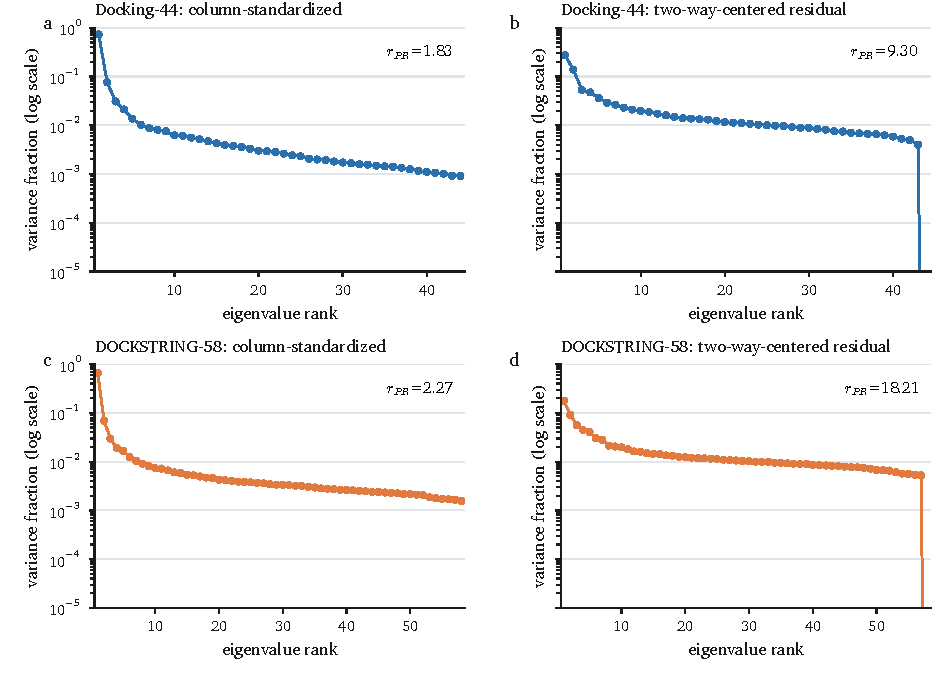
\includegraphics{figures/figS1_full_spectra.pdf}
\caption{\textbf{Full correlation-spectrum scree plots.}
\textbf{a,b}, Docking-44 column-standardized and two-way-centered residual spectra.
\textbf{c,d}, DOCKSTRING-58 column-standardized and residual spectra. Eigenvalues are divided by the
number of targets so that each spectrum sums to one. The ordinate is logarithmic. Double
centering imposes one exact zero eigenvalue; values at zero fall below the plotting range.}
\label{fig:s1}
\end{figure}

\begin{figure}[htbp]
\centering
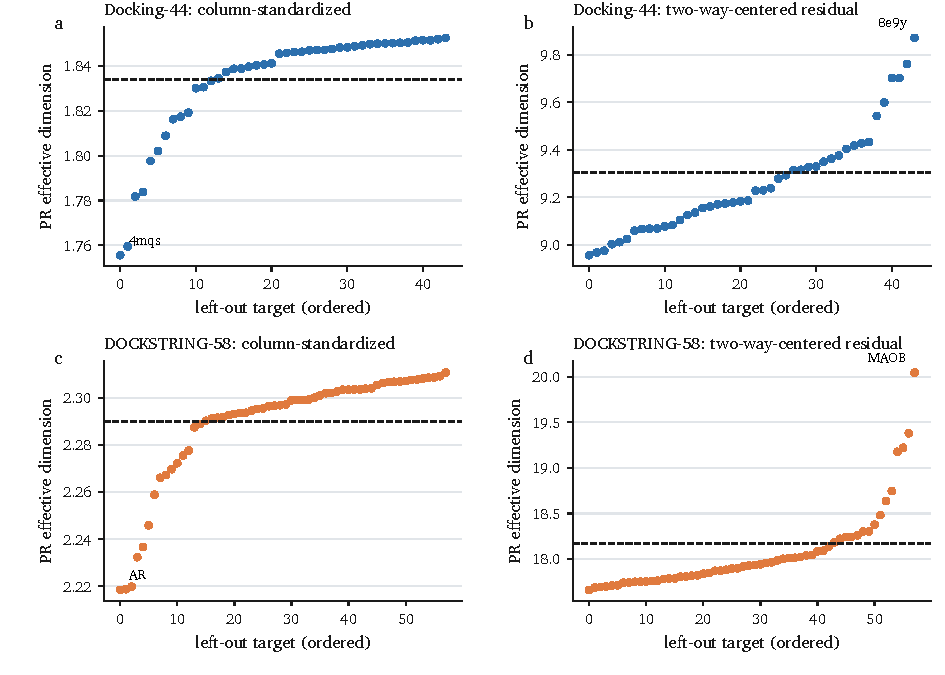
\includegraphics{figures/figS2_target_jackknife.pdf}
\caption{\textbf{Leave-one-target-out composition sensitivity.}
Each point is the PR effective dimension after deleting one target; targets are ordered by
the resulting value within each panel. Dashed lines mark the complete-panel estimate on the
same ligand support. Labels identify the most influential deletion. These ranges describe
the two observed target panels and are not confidence intervals for a target superpopulation.}
\label{fig:s2}
\end{figure}

\begin{figure}[htbp]
\centering
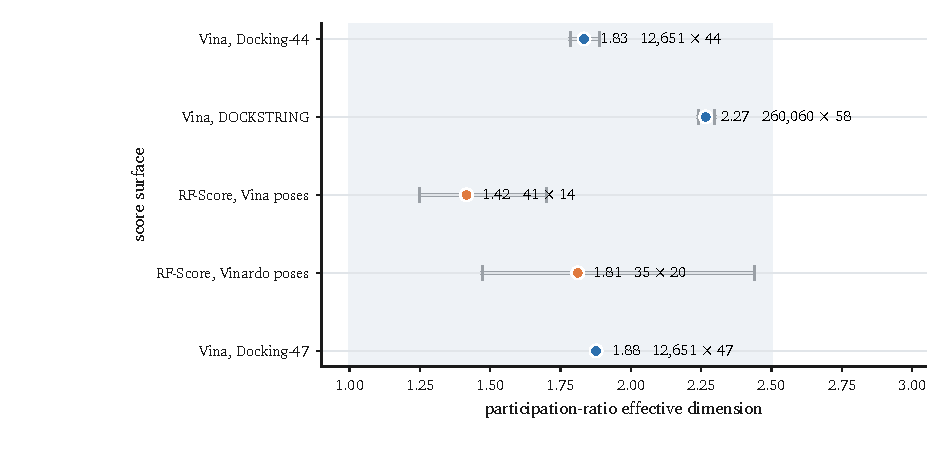
\includegraphics{figures/figS3_scoring_controls.pdf}
\caption{\textbf{Illustrative scoring-function and target-expansion sensitivities.}
PR effective dimensions and source-analysis bootstrap intervals are shown for the two large
Vina panels, RF-Score v1 on Vina poses, RF-Score v1 on Vinardo poses and the Docking-47
expansion. Point labels report ligand and target counts. The 47-target expansion is a
deterministic sensitivity and is shown without an interval. The RF-Score blocks contain only
35--41 ligands and are not large independent replications.}
\label{fig:s3}
\end{figure}

\begin{figure}[htbp]
\centering
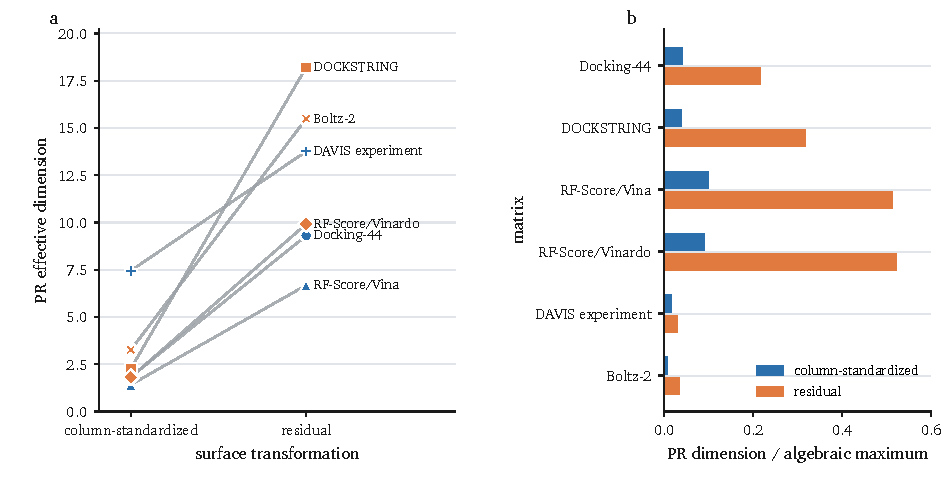
\includegraphics{figures/figS4_learned_affinity.pdf}
\caption{\textbf{Contextual centering ladder across score and affinity surfaces.}
\textbf{a}, Column-standardized and two-way-centered residual PR effective dimensions for
the two Vina matrices, two small RF-Score blocks, experimental DAVIS affinity and Boltz-2.
Lines connect the same matrix under the two transformations. \textbf{b}, Each value divided
by its algebraic maximum, $P$ before and $P-1$ after centering. The learned-affinity examples
are contextual sensitivities, not docking replications or accuracy benchmarks.}
\label{fig:s4}
\end{figure}

\begin{figure}[htbp]
\centering
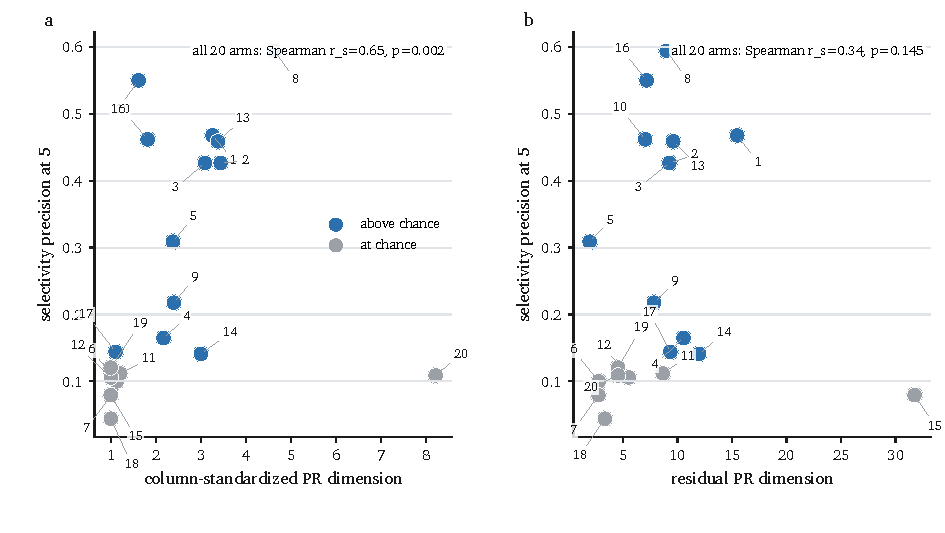
\includegraphics{figures/figS5_dti_all20.pdf}
\caption{\textbf{Exploratory DTI association on the complete 20-arm panel.}
Selectivity precision at five is plotted against the column-standardized PR effective
dimension (\textbf{a}) and the two-way-centered residual PR effective dimension (\textbf{b}).
Numbers identify arms in Table~S6; blue denotes arms above the outcome-related chance
criterion and grey denotes arms at chance. Correlations are descriptive because the arms
share data, architectures and representations.}
\label{fig:s5}
\end{figure}

\begin{figure}[htbp]
\centering
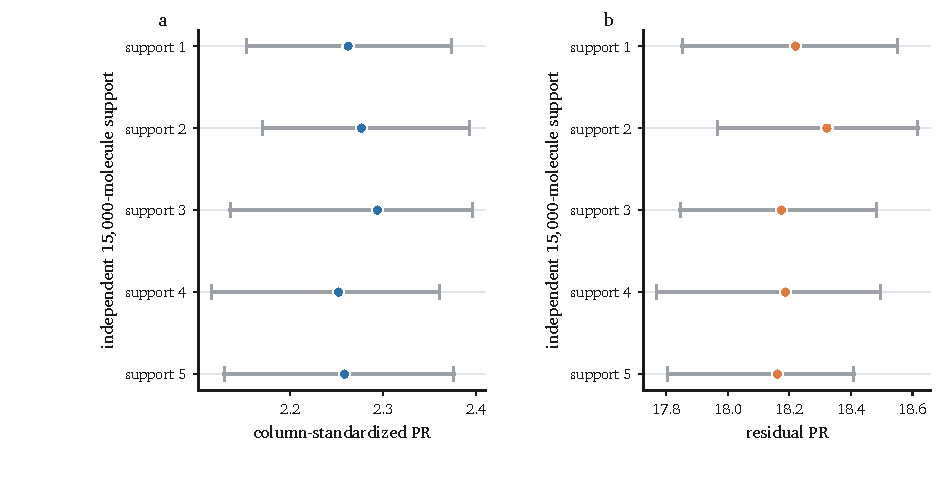
\includegraphics{figures/figS6_dockstring_supports.pdf}
\caption{\textbf{DOCKSTRING chemical-support and scaffold sensitivity.}
Each row is an independently seeded 15,000-molecule support. Points are support-specific PR
dimensions and horizontal intervals are 95\% Bemis--Murcko scaffold-cluster bootstrap
intervals from 100 replicates. \textbf{a}, Column-standardized surface; \textbf{b}, two-way-
centered residual. All estimates are conditional on the same 58 targets.}
\label{fig:s6}
\end{figure}

% Generated by analysis/make_supplement_tables.py; do not edit by hand.

\begin{landscape}
\begin{table}[!htbp]
\centering\scriptsize
\singlespacing
\setlength{\tabcolsep}{3pt}
\caption{\textbf{Large-matrix source support, analysis support and spectral summaries.} Source missingness is reported before the stated handling; the analyzed matrices are complete after Docking-44 imputation or DOCKSTRING row exclusion.}
\label{tab:s1spectral}
\begin{tabular}{lrrrrrrrrrr}
\toprule
Matrix & source $N$ & analysis $N$ & $P$ & source missing (\%) & raw PR & residual PR & raw PC1 & residual PC1 & raw $\overline{|r|}$ & residual $\overline{|r|}$ \\
\midrule
Docking-44 & 12,651 & 12,651 & 44 & 1.466 & 1.834 & 9.303 & 73.3\% & 27.4\% & 0.694 & 0.246 \\
DOCKSTRING-58 & 260,155 & 260,060 & 58 & 0.002 & 2.266 & 18.206 & 65.9\% & 17.8\% & 0.622 & 0.155 \\
\bottomrule
\end{tabular}
\end{table}

\begin{table}[!htbp]
\centering\scriptsize
\singlespacing
\setlength{\tabcolsep}{3pt}
\caption{\textbf{Large-matrix residual-spectrum sensitivity to missing-score and score-clipping handling.}}
\label{tab:s2missing}
\begin{tabular}{p{4.3cm}lrrrp{5.2cm}}
\toprule
Method & support & $N$ & $P$ & residual PR & interpretation \\
\midrule
target mean imputation & all targets & 12,651 & 44 & 9.303 & missing scores equal the observed target mean \\
target median imputation & all targets & 12,651 & 44 & 9.528 & missing scores equal the observed target median \\
observed-cell additive least-squares imputation & all targets & 12,651 & 44 & 9.663 & Each missing ligand-target interaction residual is set to zero after fitting the additive ligand and target effects on observed cells. \\
complete-case deletion & all targets & 9,297 & 44 & 13.970 & changes chemical support and is not a like-for-like imputation analysis \\
primary mean-imputed matrix restricted to complete rows & all targets & 9,297 & 44 & 13.970 & equals complete-case input exactly because these rows contain no missing cells \\
target mean imputation after target removal & without 4mqs & 12,651 & 43 & 9.433 & removes the target with the largest missing-cell count \\
target median imputation after target removal & without 4mqs & 12,651 & 43 & 9.594 & removes the target with the largest missing-cell count \\
complete cases after target removal & without 4mqs & 11,593 & 43 & 11.445 & changes both chemical and target support \\
retain positive DOCKSTRING scores & complete rows & 260,060 & 58 & 18.362 & retain 5,393 positive cells instead of clipping them at zero \\
\bottomrule
\end{tabular}
\end{table}
\end{landscape}

\begin{table}[!htbp]
\centering\scriptsize
\singlespacing
\setlength{\tabcolsep}{3pt}
\caption{\textbf{Correlation- and covariance-spectrum sensitivity.}}
\label{tab:s3covariance}
\begin{tabular}{llrrrrrr}
\toprule
Matrix & estimand & raw PR & residual PR & raw PC1 (\%) & residual PC1 (\%) & raw PCs$_{90}$ & residual PCs$_{90}$ \\
\midrule
Docking-44 & correlation & 1.834 & 9.303 & 73.3 & 27.4 & 8 & 29 \\
Docking-44 & covariance & 1.915 & 6.911 & 71.6 & 31.3 & 8 & 21 \\
DOCKSTRING-58 & correlation & 2.266 & 18.206 & 65.9 & 17.8 & 22 & 43 \\
DOCKSTRING-58 & covariance & 2.474 & 8.235 & 62.4 & 31.9 & 20 & 37 \\
\bottomrule
\end{tabular}
\end{table}

\begin{table}[!htbp]
\centering\scriptsize
\singlespacing
\setlength{\tabcolsep}{3pt}
\caption{\textbf{Residual null models on fixed 12,000-ligand supports.} Within each matrix, all three nulls use the identical deterministic ligand support; its SHA-256 row-index fingerprint is stored in the machine-readable evidence ledger.}
\label{tab:s4nulls}
\begin{tabular}{llrrrr}
\toprule
Matrix & null & observed residual PR & null median PR & draws & lower-tail $p$ \\
\midrule
Docking-44 & additive Gaussian & 9.295 & 42.400 & 500 & 0.002 \\
Docking-44 & empirical column permutation & 9.295 & 42.403 & 500 & 0.002 \\
Docking-44 & row-norm preserving & 9.295 & 42.628 & 500 & 0.002 \\
DOCKSTRING-58 & additive Gaussian & 18.158 & 56.482 & 500 & 0.002 \\
DOCKSTRING-58 & empirical column permutation & 18.158 & 56.481 & 500 & 0.002 \\
DOCKSTRING-58 & row-norm preserving & 18.158 & 56.612 & 500 & 0.002 \\
\bottomrule
\end{tabular}
\end{table}

\begin{table}[!htbp]
\centering\small
\singlespacing
\setlength{\tabcolsep}{3pt}
\caption{\textbf{Leave-one-target-out spectral composition sensitivity.}}
\label{tab:s5target}
\begin{tabular}{llrrrrl}
\toprule
Matrix & surface & full PR & minimum & median & maximum & most influential deletion \\
\midrule
Docking-44 & raw & 1.834 & 1.756 & 1.846 & 1.853 & 4mqs \\
Docking-44 & residual & 9.303 & 8.956 & 9.206 & 9.872 & 8e9y \\
DOCKSTRING-58 & raw & 2.266 & 2.218 & 2.297 & 2.311 & AR \\
DOCKSTRING-58 & residual & 18.206 & 17.662 & 17.931 & 20.045 & MAOB \\
\bottomrule
\end{tabular}
\end{table}

\begin{landscape}
\begin{table}[!htbp]
\centering\scriptsize
\singlespacing
\setlength{\tabcolsep}{3pt}
\caption{\textbf{Random and family-stratified target-subsampling sensitivity.}}
\label{tab:targetSubsampling}
\begin{tabular}{llrrrrrr}
\toprule
Matrix & design & targets & raw median & raw 2.5\% & raw 97.5\% & residual median & residual 2.5--97.5\% \\
\midrule
Docking-44 & random & 4 & 1.559 & 1.166 & 2.569 & 2.537 & 1.825--2.961 \\
Docking-44 & random & 6 & 1.629 & 1.237 & 2.517 & 3.680 & 2.453--4.583 \\
Docking-44 & random & 8 & 1.649 & 1.281 & 2.283 & 4.615 & 3.184--5.670 \\
Docking-44 & random & 12 & 1.701 & 1.340 & 2.336 & 5.938 & 4.283--7.602 \\
Docking-44 & random & 20 & 1.789 & 1.496 & 2.146 & 7.338 & 5.693--9.389 \\
Docking-44 & random & 32 & 1.841 & 1.649 & 1.993 & 8.547 & 7.447--9.994 \\
Docking-44 & random & 44 & 1.834 & 1.834 & 1.834 & 9.303 & 9.303--9.303 \\
Docking-44 & family-stratified & 12 & 1.876 & 1.609 & 2.334 & 5.834 & 4.410--7.300 \\
Docking-44 & family-stratified & 20 & 1.852 & 1.625 & 2.169 & 7.375 & 5.932--9.045 \\
Docking-44 & family-stratified & 32 & 1.835 & 1.663 & 1.978 & 8.517 & 7.269--10.014 \\
Docking-44 & family-stratified & 44 & 1.834 & 1.834 & 1.834 & 9.303 & 9.303--9.303 \\
DOCKSTRING-58 & random & 4 & 1.645 & 1.369 & 2.721 & 2.844 & 1.873--2.988 \\
DOCKSTRING-58 & random & 6 & 1.945 & 1.490 & 2.805 & 4.342 & 2.765--4.845 \\
DOCKSTRING-58 & random & 8 & 2.004 & 1.551 & 2.849 & 5.737 & 3.262--6.505 \\
DOCKSTRING-58 & random & 12 & 2.074 & 1.664 & 2.732 & 8.051 & 5.198--9.442 \\
DOCKSTRING-58 & random & 20 & 2.180 & 1.746 & 2.790 & 11.196 & 7.669--14.391 \\
DOCKSTRING-58 & random & 32 & 2.233 & 1.958 & 2.537 & 14.367 & 10.905--18.012 \\
DOCKSTRING-58 & random & 44 & 2.240 & 2.043 & 2.400 & 16.467 & 13.717--20.031 \\
DOCKSTRING-58 & random & 58 & 2.266 & 2.266 & 2.266 & 18.206 & 18.206--18.206 \\
DOCKSTRING-58 & family-stratified & 6 & 1.947 & 1.548 & 2.545 & 4.538 & 3.021--4.847 \\
DOCKSTRING-58 & family-stratified & 8 & 2.024 & 1.617 & 2.674 & 5.983 & 3.718--6.594 \\
DOCKSTRING-58 & family-stratified & 12 & 2.093 & 1.657 & 2.628 & 8.363 & 5.384--9.713 \\
DOCKSTRING-58 & family-stratified & 20 & 2.217 & 1.875 & 2.624 & 11.401 & 7.414--14.186 \\
DOCKSTRING-58 & family-stratified & 32 & 2.247 & 2.051 & 2.548 & 14.612 & 11.227--17.975 \\
DOCKSTRING-58 & family-stratified & 44 & 2.273 & 2.087 & 2.429 & 16.850 & 14.007--19.743 \\
DOCKSTRING-58 & family-stratified & 58 & 2.266 & 2.266 & 2.266 & 18.206 & 18.206--18.206 \\
\bottomrule
\end{tabular}
\end{table}
\end{landscape}

\begin{table}[!htbp]
\centering\scriptsize
\singlespacing
\setlength{\tabcolsep}{3pt}
\caption{\textbf{Complete docking-by-experimental estimand decomposition on the common 20 kinases.} Each $\Delta_D^{F/M}$ cell gives the full-reference increment followed by the increment on the fixed 15,000-ligand support; $p_L$ denotes the paired target-label QAP for the first and $p_M$ the transformation-matched independent-column null for the second. Differences were calculated from unrounded correlations and can therefore differ slightly from subtraction of the displayed entries.}
\label{tab:s6factorial}
\resizebox{\linewidth}{!}{%
\begin{tabular}{lrrrrrrrrrrrr}
\toprule
Panel & $N$ & $D_R/E_R$ & $D_R/E_C$ & $D_C/E_R$ & $D_C/E_C$ & $\Delta_D^{F/M}\mid E_R$ & $p_L$ & $p_M$ & $\Delta_D^{F/M}\mid E_C$ & $p_L$ & $p_M$ & interaction \\
\midrule
DAVIS & 72 & 0.050 & 0.263 & 0.219 & 0.280 & +0.168/+0.162 & 0.01512 & 0.00300 & +0.016/+0.010 & 0.335 & 0.690 & -0.152 \\
PKIS2 & 645 & -0.215 & 0.243 & 0.033 & 0.287 & +0.249/+0.243 & 0.00152 & 0.00050 & +0.044/+0.034 & 0.146 & 0.172 & -0.205 \\
PKIS1 & 360 & -0.159 & 0.173 & 0.059 & 0.174 & +0.218/+0.215 & 0.00536 & 0.00050 & +0.001/-0.006 & 0.462 & 0.513 & -0.217 \\
KiRHub & 92 & -0.029 & 0.276 & 0.235 & 0.322 & +0.264/+0.261 & 0.00008 & 0.00050 & +0.045/+0.041 & 0.126 & 0.073 & -0.219 \\
\bottomrule
\end{tabular}
}
\end{table}

\begin{table}[!htbp]
\centering\scriptsize
\singlespacing
\setlength{\tabcolsep}{3pt}
\caption{\textbf{Path-dependent allocation of the joint raw/raw-to-centred/centred change.}}
\label{tab:s7paths}
\begin{tabular}{lrrrrrr}
\toprule
Panel & joint change & experiment-first $\Delta_E$ & final $\Delta_D$ & sequential $E$ fraction & path-averaged $E$ share & path-averaged $D$ share \\
\midrule
DAVIS & 0.230 & 0.213 & 0.016 & 92.9\% & 0.137 (59.8\%) & 0.092 (40.2\%) \\
PKIS2 & 0.502 & 0.459 & 0.044 & 91.3\% & 0.356 (70.9\%) & 0.146 (29.1\%) \\
PKIS1 & 0.333 & 0.332 & 0.001 & 99.7\% & 0.223 (67.1\%) & 0.109 (32.9\%) \\
KiRHub & 0.351 & 0.305 & 0.045 & 87.0\% & 0.196 (55.8\%) & 0.155 (44.2\%) \\
\bottomrule
\end{tabular}
\end{table}

\begin{table}[!htbp]
\centering\scriptsize
\singlespacing
\setlength{\tabcolsep}{3pt}
\caption{\textbf{Strict common-20 reference-library sensitivity for centred docking versus centred experiment.}}
\label{tab:referenceSupport}
\begin{tabular}{lrrrr}
\toprule
Panel & full 259,579-row reference & same-scaffold-excluded & change & five 15,000-row supports \\
\midrule
DAVIS & 0.280 & 0.279 & -0.0009 & 0.271--0.285 \\
PKIS2 & 0.287 & 0.287 & -0.0006 & 0.277--0.290 \\
PKIS1 & 0.174 & 0.172 & -0.0017 & 0.167--0.176 \\
KiRHub & 0.322 & -- & -- & 0.312--0.326 \\
\bottomrule
\end{tabular}
\end{table}

\begin{table}[!htbp]
\centering\scriptsize
\singlespacing
\setlength{\tabcolsep}{3pt}
\caption{\textbf{Four-panel experimental geometry agreement under complementary null models.}}
\label{tab:s8experimental}
\begin{tabular}{p{6.2cm}rrp{5.4cm}}
\toprule
Quantity & raw & centred & interpretation \\
\midrule
Mean of six pairwise panel concordances & 0.632 & 0.763 & absolute centred target-label QAP $p=2.0e-05$; transformation-matched absolute $p=5.0e-04$ \\
Centred minus raw & \multicolumn{2}{c}{+0.131} & global target-label network QAP $p=0.002$; transformation-matched independent-column null $p=0.947$ \\
Transformation-matched null mean & -0.000 & 0.179 & mean mechanical increment +0.179; its raw baseline is not conditioned on the observed 0.632 \\
KiRHub versus mean of DAVIS/PKIS2/PKIS1 & -- & 0.834 & 0.817 after removing 11 exact-name overlaps; 0.802 after sequence adjustment \\
\bottomrule
\end{tabular}
\end{table}

\begin{table}[!htbp]
\centering\scriptsize
\singlespacing
\setlength{\tabcolsep}{3pt}
\caption{\textbf{Censoring-aware DAVIS sensitivity on the fixed kinase panel.} Each row compares centred DOCKSTRING target-pair geometry with the stated DAVIS geometry; probabilities use complete target-label permutations. The binary endpoint records whether Kd was measured below the released 10,000-nM limit, not quantitative affinity.}
\label{tab:davisCensoring}
\begin{tabular}{p{6.1cm}rrr}
\toprule
DAVIS representation & targets & Spearman $\rho$ & QAP $p$ \\
\midrule
continuous pKd, all targets & 20 & 0.280 & 0.005 \\
binary above-pKd-5-floor status, all targets & 20 & 0.292 & 0.004 \\
continuous pKd; at least 5 values above floor per target & 18 & 0.255 & 0.010 \\
continuous pKd; at least 10 values above floor per target & 16 & 0.210 & 0.030 \\
continuous pKd; at least 15 values above floor per target & 12 & 0.229 & 0.049 \\
\bottomrule
\end{tabular}
\end{table}

\begin{table}[!htbp]
\centering\scriptsize
\singlespacing
\setlength{\tabcolsep}{3pt}
\caption{\textbf{Fixed experimental target-pair endpoint was selected before KiRHub inspection but not preregistered.}}
\label{tab:s9lockedPairs}
\begin{tabular}{p{1.7cm}p{2.0cm}p{2.5cm}p{1.8cm}p{1.8cm}p{1.8cm}p{1.8cm}}
\toprule
Target A & Target B & panels in top decile & DAVIS percentile & PKIS2 percentile & PKIS1 percentile & mean percentile \\
\midrule
ABL1 & KDR & 2 & 0.434 & 0.955 & 0.934 & 0.775 \\
ABL1 & LCK & 3 & 0.982 & 0.934 & 0.971 & 0.962 \\
ABL1 & SRC & 2 & 0.961 & 0.887 & 0.982 & 0.943 \\
AKT1 & AKT2 & 3 & 0.997 & 0.997 & 0.997 & 0.997 \\
AKT1 & MAPK1 & 2 & 0.934 & 0.950 & 0.850 & 0.911 \\
AKT1 & MAPKAPK2 & 2 & 0.955 & 0.876 & 0.961 & 0.931 \\
AKT1 & ROCK1 & 3 & 0.945 & 0.961 & 0.908 & 0.938 \\
AKT2 & MAPK1 & 2 & 0.939 & 0.945 & 0.861 & 0.915 \\
AKT2 & MAPKAPK2 & 3 & 0.966 & 0.966 & 0.955 & 0.962 \\
CSF1R & KDR & 2 & 0.929 & 0.982 & 0.792 & 0.901 \\
CSF1R & KIT & 3 & 0.992 & 0.992 & 0.976 & 0.987 \\
IGF1R & MAPK1 & 2 & 0.918 & 0.939 & 0.803 & 0.887 \\
KDR & KIT & 2 & 0.971 & 0.971 & 0.882 & 0.941 \\
LCK & SRC & 3 & 0.976 & 0.987 & 0.987 & 0.983 \\
MAPK1 & MAPKAPK2 & 3 & 0.987 & 0.976 & 0.966 & 0.976 \\
\bottomrule
\end{tabular}
\end{table}

\begin{table}[!htbp]
\centering\small
\singlespacing
\setlength{\tabcolsep}{3pt}
\caption{\textbf{KiRHub evaluation and structural controls for the fixed 15-of-190 target-pair endpoint.} The endpoint was defined before KiRHub inspection but not preregistered. Absolute-predictor rows use target-label QAP. The contrast rows show how the same centred-minus-raw increment is assessed under target-label and transformation-matched nulls; the absolute centred KiRHub predictor also exceeded the transformation-matched null ($p=0.00050$ for both metrics).}
\label{tab:s10structure}
\begin{tabular}{p{5.3cm}rrrr}
\toprule
Quantity & AUROC/value & AUROC null $p$ & AP/value & AP null $p$ \\
\midrule
raw KiRHub experimental geometry & 0.803 & 0.00014 & 0.597 & 0.00002 \\
centred KiRHub experimental geometry & 0.963 & 0.00002 & 0.694 & 0.00002 \\
centred minus raw KiRHub, target-label QAP & +0.160 & 0.04928 & +0.097 & 0.02306 \\
centred minus raw KiRHub, transformation-matched null & +0.160 & 0.74763 & +0.097 & 0.99650 \\
Holm-adjusted target-label gain probabilities & -- & 0.04928 & -- & 0.04612 \\
receptor-domain sequence identity & 0.718 & 0.007 & 0.426 & 2.0e-05 \\
KLIFS pocket identity & 0.708 & 0.010 & 0.486 & 2.0e-05 \\
same KLIFS group & 0.651 & 0.043 & 0.126 & 0.016 \\
same KLIFS family & 0.597 & 0.001 & 0.192 & 0.002 \\
raw Vina geometry & 0.597 & 0.155 & 0.236 & 0.011 \\
centred Vina geometry & 0.710 & 0.007 & 0.301 & 0.001 \\
\bottomrule
\end{tabular}
\end{table}

\begin{table}[!htbp]
\centering\scriptsize
\singlespacing
\setlength{\tabcolsep}{3pt}
\caption{\textbf{Chemical-group-held-out predictive decomposition of the residual docking surfaces.} Every target offset, residual target scale, descriptor scale and regression coefficient was fitted within the training fold. The seven descriptors were heavy-atom count, molecular weight, Labute ASA, TPSA, cLogP, rotatable-bond count and ring count. The change in mean squared target correlation is predictive, not causal attribution.}
\label{tab:descriptorDecomposition}
\resizebox{\linewidth}{!}{%
\begin{tabular}{lrrrrrr}
\toprule
Matrix & ligands & chemical groups & residual PR before & PR after descriptor removal & mean $r^2$ reduction & residual-PC1 out-of-fold $R^2$ \\
\midrule
Docking-44 & 12,651 & 8,150 & 9.294 & 14.746 & 46.9\% & 0.586 \\
DOCKSTRING-58 & 15,000 & 11,905 & 17.923 & 28.466 & 53.6\% & 0.687 \\
\bottomrule
\end{tabular}
}
\end{table}

\begin{table}[!htbp]
\centering\scriptsize
\singlespacing
\setlength{\tabcolsep}{3pt}
\caption{\textbf{Spectral concentration under six non-Vina scoring functions on identical fixed DOCKSTRING poses.} Every scorer sees the same 2,000-ligand by 9-target pose block; only the scoring function changes. The four prediction criteria were fixed before the non-Vina scores were inspected: raw PC1 fraction at least 0.50, cosine to the uniform target direction at least 0.95 with no negative loading, raw participation ratio no greater than half the target count, and a centring-induced participation-ratio increase whose 95\% cluster-bootstrap interval excludes zero. These criteria are a weak bar: a one-factor surface with no target identity satisfies all four, so meeting them evidences a shared positive ligand axis and nothing finer. Two margins sit inside bootstrap noise: released Vina passes the cosine criterion at 0.9501, and PLECscore exceeds the participation-ratio threshold at the point estimate with an interval that spans it, whereas its PC1 failure holds in every replicate. Scores are not clipped, because clipping only the Vina-family columns would be asymmetric. On a separate 512-ligand fixed-pose within-Vina attribution, gauss2 supplied 0.715 of the shared-axis covariance and 0.525 of the residual Frobenius inner product. These are signed arithmetic attributions without resampling uncertainty; term deletion on Vina-selected poses is not an independent redocking ablation.}
\label{tab:scorerTransport}
\resizebox{\linewidth}{!}{%
\begin{tabular}{llrrrrrl}
\toprule
Scorer & family & raw PC1 & raw PR & centred PR & PR increase & uniform cosine & criteria met \\
\midrule
released vina & Vina family & 57.3\% & 2.74 & 5.12 & 2.38 & 0.9501 & all four \\
smina vina & Vina family & 57.7\% & 2.71 & 5.13 & 2.42 & 0.9546 & all four \\
vinardo & empirical & 56.7\% & 2.81 & 5.74 & 2.93 & 0.9668 & all four \\
rfscore v1 & machine learned & 63.5\% & 2.34 & 6.44 & 4.10 & 0.9587 & all four \\
rfscore v2 & machine learned & 66.9\% & 2.13 & 5.65 & 3.52 & 0.9535 & all four \\
rfscore v3 & machine learned & 63.0\% & 2.37 & 6.00 & 3.63 & 0.9562 & all four \\
nnscore & machine learned & 52.6\% & 3.21 & 6.79 & 3.59 & 0.9730 & all four \\
plecscore linear & machine learned & 41.4\% & 4.59 & 7.47 & 2.87 & 0.9858 & PC1 fails \\
\bottomrule
\end{tabular}
}
\end{table}

\begin{table}[!htbp]
\centering\scriptsize
\singlespacing
\setlength{\tabcolsep}{3pt}
\caption{\textbf{Rank-matched ligand-feature controls on the fixed common-20 kinase support.} Each seven-dimensional basis receives separate target-specific coefficients in five chemical-group-held-out folds. Mean out-of-fold target $R^2$ measures held-out predictive performance. Operational reduction is $1-\overline{r^2}_{\rm error}/\overline{r^2}_{\rm observed}$; it is non-additive and is not a share of correlation, covariance or variance explained. The four final columns are scale-free Spearman agreements between the fitted-component target-correlation map and each experimental map over the same 190 edges. The hash arm has negligible held-out predictive performance but appreciable map agreement, so component-map agreement alone cannot identify a feature-specific mechanism or mediation path.}
\label{tab:descriptorRankMatched}
\resizebox{\linewidth}{!}{%
\begin{tabular}{p{4.1cm}rrrrrr}
\toprule
Seven-dimensional basis & mean OOF target $R^2$ & operational reduction & DAVIS $\rho$ & PKIS2 $\rho$ & PKIS1 $\rho$ & KiRHub $\rho$ \\
\midrule
physicochemical descriptors & 0.1068 & 23.361\% & 0.256 & 0.218 & 0.097 & 0.288 \\
count-Morgan random projection (locked seed) & 0.0903 & 23.765\% & 0.299 & 0.279 & 0.139 & 0.359 \\
stable ligand-identity hash nuisance & $-3.63\times10^{-5}$ & 0.002\% & 0.248 & 0.250 & 0.103 & 0.348 \\
\bottomrule
\end{tabular}
}
\end{table}

\begin{table}[!htbp]
\centering\scriptsize
\singlespacing
\setlength{\tabcolsep}{3pt}
\caption{\textbf{Algorithmic basis sensitivity for the rank-matched controls.} The count-Morgan column spans 20 deterministic unnormalised count-fingerprint projections; the row-permuted column spans 20 deterministic permutations of the same standardised physicochemical feature cloud, which destroy the ligand--feature assignment. Ranges are across fixed seeds, not confidence intervals or chemical-space uncertainty. A scale-free component map can remain concordant when held-out predictive performance is effectively null because every nuisance basis is projected separately onto each target and correlation discards component scale. These rows therefore cannot be read as mediation or feature-specific biological attribution.}
\label{tab:descriptorAlgorithmicControls}
\resizebox{\linewidth}{!}{%
\begin{tabular}{p{5.1cm}rrr}
\toprule
Quantity & physicochemical point & count-Morgan 20-seed range & row-permuted-physicochemical 20-seed range \\
\midrule
mean OOF target $R^2$ & 0.107 & 0.081~--~0.098 & -0.00005~--~-0.00002 \\
operational reduction & 0.234 & 0.176~--~0.260 & -0.00007~--~0.00007 \\
component-map agreement: DAVIS & 0.256 & 0.236~--~0.336 & 0.034~--~0.489 \\
component-map agreement: PKIS2 & 0.218 & 0.238~--~0.322 & 0.025~--~0.452 \\
component-map agreement: PKIS1 & 0.097 & 0.100~--~0.173 & -0.072~--~0.401 \\
component-map agreement: KiRHub & 0.288 & 0.299~--~0.404 & 0.030~--~0.564 \\
\bottomrule
\end{tabular}
}
\end{table}

\begin{landscape}
\begin{table}[!htbp]
\centering\scriptsize
\singlespacing
\setlength{\tabcolsep}{3pt}
\caption{\textbf{Exploratory low- versus high-molecular-weight transfer of the docking target-pair maps.} Parenthesized intervals for the cross-band and descriptor-adjusted contrasts are paired chemical-group bootstrap central 95\% intervals. Within-band controls split the low- and high-MW restrictions separately, keep whole chemical groups disjoint, and report raw/residual means over 200 MW-stratified repeated splits; their full 2.5--97.5\% composition-sensitivity ranges are in the accompanying machine-readable CSV and are not population confidence intervals. The size-matched control uses random disjoint supports matching the observed low/high row counts; the MW-matched control uses chemically disjoint supports with closely matched molecular-weight distributions. Descriptor adjustment is five-fold group-held-out and fold-local. The final column gives the residual cross-band range over six independently seeded fixed DOCKSTRING supports and is an algorithmic support sensitivity, not an interval.}
\label{tab:dockingChemicalDomain}
\resizebox{\linewidth}{!}{%
\begin{tabular}{lrrrrrrrr}
\toprule
Matrix & raw cross-band $\rho$ (95\%) & residual cross-band $\rho$ (95\%) & within-low raw/residual & within-high raw/residual & size-matched residual & MW-matched residual & adjusted residual $\rho$ (95\%) & six-seed residual range \\
\midrule
Docking-44 & 0.227 (0.209--0.246) & 0.205 (0.185--0.219) & 0.989/0.980 & 0.989/0.978 & 0.991 & 0.991 & 0.489 (0.446--0.515) & -- \\
DOCKSTRING-58 & 0.409 (0.384--0.432) & 0.351 (0.326--0.363) & 0.991/0.978 & 0.979/0.966 & 0.990 & 0.994 & 0.437 (0.406--0.458) & 0.325--0.361 \\
\bottomrule
\end{tabular}
}
\end{table}
\end{landscape}

\begin{landscape}
\begin{table}[!htbp]
\centering\scriptsize
\singlespacing
\setlength{\tabcolsep}{3pt}
\caption{\textbf{Post-hoc descriptor-family sensitivity of residual-map transport.} Each row compares groups at the inclusive 25th- and 75th-percentile thresholds of one of the seven already inspected descriptors on the row-centred residual surface; all boundary ties are retained. The common within-dataset MW-matched reference is the mean agreement between chemically disjoint supports with closely matched molecular-weight distributions; it is not separately descriptor-matched. All 14 observed agreements are below that dataset-level reference. The molecular-size family supplies the three lowest agreements in both panels, but this descriptive ordering neither identifies a unique descriptor mechanism nor constitutes multiplicity-adjusted inference.}
\label{tab:descriptorFamilyStratification}
\begin{tabular}{lllrrrrrr}
\toprule
Matrix & stratifier & family & low/high $N$ & residual PR (low) & residual PR (high) & map $\rho$ & sign flips (\%) & MW-matched control $\rho$ \\
\midrule
Docking-44 & heavy-atom count & molecular size & 3,545/3,523 & 14.54 & 9.90 & 0.207 & 42.4 & 0.991 \\
Docking-44 & molecular weight & molecular size & 3,163/3,163 & 13.62 & 10.15 & 0.205 & 42.5 & 0.991 \\
Docking-44 & Labute ASA & molecular size & 3,163/3,163 & 14.16 & 10.16 & 0.200 & 44.0 & 0.991 \\
Docking-44 & TPSA & polarity & 3,163/3,167 & 10.47 & 8.62 & 0.753 & 20.8 & 0.991 \\
Docking-44 & cLogP & lipophilicity & 3,164/3,163 & 8.44 & 9.65 & 0.887 & 13.1 & 0.991 \\
Docking-44 & rotatable bonds & flexibility & 3,736/3,168 & 8.74 & 9.31 & 0.789 & 20.3 & 0.991 \\
Docking-44 & ring count & ring topology & 4,537/4,349 & 12.42 & 9.39 & 0.703 & 22.6 & 0.991 \\
DOCKSTRING-58 & heavy-atom count & molecular size & 4,367/3,817 & 20.03 & 23.78 & 0.361 & 36.3 & 0.994 \\
DOCKSTRING-58 & molecular weight & molecular size & 3,751/3,750 & 19.55 & 23.80 & 0.351 & 36.7 & 0.994 \\
DOCKSTRING-58 & Labute ASA & molecular size & 3,750/3,750 & 20.06 & 23.62 & 0.322 & 37.7 & 0.994 \\
DOCKSTRING-58 & TPSA & polarity & 3,755/3,750 & 17.12 & 19.61 & 0.787 & 19.7 & 0.994 \\
DOCKSTRING-58 & cLogP & lipophilicity & 3,750/3,750 & 18.69 & 19.40 & 0.822 & 17.5 & 0.994 \\
DOCKSTRING-58 & rotatable bonds & flexibility & 6,154/4,352 & 17.27 & 18.45 & 0.831 & 18.5 & 0.994 \\
DOCKSTRING-58 & ring count & ring topology & 8,376/6,624 & 19.97 & 22.04 & 0.803 & 18.2 & 0.994 \\
\bottomrule
\end{tabular}
\end{table}
\end{landscape}

\begin{table}[!htbp]
\centering\small
\singlespacing
\setlength{\tabcolsep}{3pt}
\caption{\textbf{Continuous Vina association after sequence and pocket adjustment.}}
\label{tab:s11partial}
\begin{tabular}{lrrr}
\toprule
Experimental endpoint & partial Spearman & unrestricted QAP $p$ & within-KLIFS-group QAP $p$ \\
\midrule
mean of DAVIS/PKIS2/PKIS1 & 0.225 & 0.014 & 0.197 \\
KiRHub & 0.280 & 0.007 & 0.166 \\
\bottomrule
\end{tabular}
\end{table}

\begin{table}[!htbp]
\centering\small
\singlespacing
\setlength{\tabcolsep}{3pt}
\caption{\textbf{Chemical-support and centering-panel sensitivities.}}
\label{tab:s12support}
\begin{tabular}{lrrrrrr}
\toprule
Panel & low/high-MW $\rho$ & random mean & matched $p$ & local-20 $\rho$ & all-58 $\rho$ & all-58 minus local \\
\midrule
DAVIS & 0.531 & 0.619 & 0.173 & 0.280 & 0.261 & -0.019 \\
PKIS2 & 0.333 & 0.845 & 1.0e-03 & 0.287 & 0.274 & -0.013 \\
PKIS1 & 0.547 & 0.833 & 1.0e-03 & 0.174 & 0.166 & -0.008 \\
KiRHub & -- & -- & -- & 0.322 & 0.302 & -0.019 \\
\bottomrule
\end{tabular}
\end{table}

\begin{table}[!htbp]
\centering\small
\singlespacing
\setlength{\tabcolsep}{3pt}
\caption{\textbf{Recovery of each full source-library target map from sampled ligands.}}
\label{tab:s13recovery}
\begin{tabular}{lrrrr}
\toprule
Matrix & ligands & mean Spearman & 2.5--97.5\% range & chemical-group-held-out mean \\
\midrule
Docking-44 & 50 & 0.813 & 0.657--0.901 & -- \\
Docking-44 & 100 & 0.898 & 0.772--0.946 & -- \\
Docking-44 & 200 & 0.942 & 0.898--0.962 & 0.927 \\
Docking-44 & 500 & 0.976 & 0.961--0.984 & 0.959 \\
Docking-44 & 1,000 & 0.987 & 0.977--0.991 & -- \\
Docking-44 & 2,000 & 0.994 & 0.991--0.996 & -- \\
Docking-44 & 5,000 & 0.998 & 0.997--0.999 & -- \\
DOCKSTRING-58 & 50 & 0.766 & 0.665--0.822 & -- \\
DOCKSTRING-58 & 100 & 0.861 & 0.808--0.896 & -- \\
DOCKSTRING-58 & 200 & 0.918 & 0.885--0.938 & 0.916 \\
DOCKSTRING-58 & 500 & 0.965 & 0.951--0.972 & 0.958 \\
DOCKSTRING-58 & 1,000 & 0.982 & 0.977--0.986 & -- \\
DOCKSTRING-58 & 2,000 & 0.991 & 0.987--0.992 & -- \\
DOCKSTRING-58 & 5,000 & 0.996 & 0.995--0.997 & -- \\
\bottomrule
\end{tabular}
\end{table}

\begin{table}[!htbp]
\centering\small
\singlespacing
\setlength{\tabcolsep}{3pt}
\caption{\textbf{Overlap between the two independently sourced Vina panels.}}
\label{tab:s14overlap}
\begin{tabular}{p{7.4cm}rp{6.4cm}}
\toprule
Overlap definition & count & boundary \\
\midrule
full Standard InChIKeys & 582 & exact structure layer \\
14-character connectivity blocks & 804 & merges stereochemical and protonation suffixes \\
non-empty Bemis--Murcko scaffolds & 1,340 & scaffold-level chemical overlap \\
mapped protein identities & 9 & 7 map to human receptors \\
same receptor structures & 3 & exact structure and chain used in both panels \\
\bottomrule
\end{tabular}
\end{table}

\begin{table}[!htbp]
\centering\scriptsize
\singlespacing
\setlength{\tabcolsep}{3pt}
\caption{\textbf{Chemical overlap among the three experimental panels with released structures.} Full keys are recomputed Standard InChIKeys; connectivity is the 14-character block; Murcko intersections exclude empty scaffolds.}
\label{tab:experimentalPanelOverlap}
\begin{tabular}{lrrrrr}
\toprule
Panel pair & $N_A$ & $N_B$ & full keys & connectivity & Murcko \\
\midrule
DAVIS--PKIS2 & 72 & 645 & 3 & 6 & 10 \\
DAVIS--PKIS1 & 72 & 360 & 1 & 1 & 5 \\
PKIS2--PKIS1 & 645 & 360 & 7 & 7 & 43 \\
\midrule
\multicolumn{6}{p{14.2cm}}{Three-panel intersection: 0 full keys, 0 connectivity blocks and 3 non-empty Murcko scaffolds. KiRHub has 92 rows but no released structures; 11 exact normalized-name overlaps with DAVIS were removed in a sensitivity ($\rho=0.817$). No PKIS--KiRHub identity claim is made.} \\
\bottomrule
\end{tabular}
\end{table}

\begin{table}[!htbp]
\centering\scriptsize
\singlespacing
\setlength{\tabcolsep}{3pt}
\caption{\textbf{Matched 74-ligand by 6-target ChEMBL--docking spectral comparison.}}
\label{tab:s15matched}
\begin{tabular}{p{3.0cm}p{2.0cm}p{2.2cm}p{2.6cm}p{4.3cm}}
\toprule
Surface & docking PR & experiment PR & experiment minus docking & paired ligand-bootstrap 95\% interval \\
\midrule
column-standardized & 1.827 & 3.833 & +2.006 & 1.174~--~2.673 \\
two-way residual & 3.646 & 4.128 & +0.483 & -0.071~--~0.921 \\
\bottomrule
\end{tabular}
\end{table}

\begin{table}[!htbp]
\centering\scriptsize
\singlespacing
\setlength{\tabcolsep}{3pt}
\caption{\textbf{Broad DOCKSTRING--ChEMBL observed-pair benchmark.} The 6,557 retained ligands provide at least two observed targets; 6,480 have a non-tied pair and enter the mean per-ligand endpoint. The docking and external experimental priors are ligand-invariant target means fitted after excluding all evaluation ligands. The cohort outcome prior is refitted after excluding each evaluated ligand's complete Bemis--Murcko scaffold cluster and is a benchmark-fitted, non-deployable reference. Chemical intervals are the conservative union of Murcko- and Butina-cluster 95\% intervals. Target-centred and two-way-centred unscaled scores are exactly rank-identical because they differ only by a ligand-wise constant. The final row is the paired absolute-Vina-minus-docking-prior contrast on the same evaluated ligands, not an additional representation.}
\label{tab:broadRanking}
\resizebox{\linewidth}{!}{%
\begin{tabular}{p{4.4cm}rrrrrr}
\toprule
Representation & mean per-ligand concordance & pair-weighted & top-1 & evaluated ligands & pairs & chemical-cluster 95\% interval \\
\midrule
ligand-invariant docking target prior & 0.524 & 0.514 & 0.444 & 6,480 & 25,214 & 0.495~--~0.552 \\
ligand-invariant external experimental prior & 0.480 & 0.495 & 0.417 & 6,480 & 25,214 & 0.451~--~0.511 \\
scaffold-cross-fitted cohort outcome prior & 0.604 & 0.572 & 0.521 & 6,480 & 25,214 & 0.573~--~0.632 \\
absolute Vina & 0.537 & 0.528 & 0.468 & 6,480 & 25,214 & 0.518~--~0.556 \\
target-centred, unscaled & 0.533 & 0.528 & 0.471 & 6,480 & 25,214 & 0.514~--~0.552 \\
two-way-centred, unscaled & 0.533 & 0.528 & 0.471 & 6,480 & 25,214 & 0.515~--~0.552 \\
column-standardised Vina & 0.530 & 0.526 & 0.467 & 6,480 & 25,214 & 0.511~--~0.550 \\
target-centred, residual-SD scaled & 0.526 & 0.519 & 0.463 & 6,480 & 25,214 & 0.507~--~0.545 \\
scaled two-way residual & 0.529 & 0.527 & 0.467 & 6,480 & 25,214 & 0.511~--~0.549 \\
\midrule
paired: absolute Vina minus docking target prior & +0.013 & -- & -- & 6,480 & 25,214 & -0.011~--~0.038 \\
\bottomrule
\end{tabular}
}
\end{table}

\begin{table}[!htbp]
\centering\scriptsize
\singlespacing
\setlength{\tabcolsep}{4pt}
\caption{\textbf{Endpoint-restricted DOCKSTRING--ChEMBL ranking arms.} Every row retains the externally fitted docking transformation and changes only the experimental support/endpoint contract. The contrast is scaled two-way residual minus absolute Vina. Chemical 95\% intervals are conservative unions over Murcko and Butina cluster bootstraps and remain conditional on target labels. Target intervals are delete-one-target jackknife normal approximations for the fixed panel; they address panel composition rather than chemical sampling. Separate Ki, Kd, IC50 and EC50 arms are exploratory and unadjusted for multiplicity. Panel c audits endpoint provenance without changing the human binding Ki/Kd estimand: each cell remains the pooled median over all eligible records, and any pair involving a cell with both Ki and Kd records is reported separately rather than assigned an artificial endpoint label.}
\label{tab:endpointRanking}
\textbf{a. Support and representation estimates}\par\smallskip
\resizebox{\textwidth}{!}{%
\begin{tabular}{p{4.3cm}rrrrrrrr}
\toprule
Endpoint contract & retained & evaluated & targets & cells & pairs & absolute & column-standardised & residual \\
\midrule
all exact-relation endpoints (broad primary) & 6,557 & 6,480 & 31 & 18,020 & 25,214 & 0.537 & 0.530 & 0.529 \\
human binding Ki/Kd & 1,056 & 1,049 & 31 & 2,783 & 3,955 & 0.559 & 0.512 & 0.520 \\
single endpoint: Ki & 1,608 & 1,594 & 31 & 5,891 & 12,895 & 0.549 & 0.512 & 0.516 \\
single endpoint: Kd & 160 & 160 & 24 & 763 & 2,534 & 0.488 & 0.532 & 0.526 \\
single endpoint: IC50 & 4,701 & 4,647 & 30 & 11,301 & 9,963 & 0.539 & 0.536 & 0.533 \\
single endpoint: EC50 & 439 & 424 & 17 & 882 & 435 & 0.581 & 0.620 & 0.594 \\
\bottomrule
\end{tabular}
}
\par\medskip
\textbf{b. Paired scaled-residual-minus-absolute contrasts}\par\smallskip
\begin{tabular}{p{5.3cm}rrr}
\toprule
Endpoint contract & point difference & chemical-cluster 95\% & target-jackknife 95\% \\
\midrule
all exact-relation endpoints (broad primary) & -0.008 & -0.022~--~0.006 & -0.056~--~0.030 \\
human binding Ki/Kd & -0.040 & -0.091~--~0.003 & -0.133~--~0.029 \\
single endpoint: Ki & -0.033 & -0.069~--~-0.005 & -- \\
single endpoint: Kd & +0.038 & -0.008~--~0.080 & -- \\
single endpoint: IC50 & -0.006 & -0.022~--~0.011 & -- \\
single endpoint: EC50 & +0.013 & -0.013~--~0.042 & -- \\
\bottomrule
\end{tabular}
\par\medskip
\textbf{c. Endpoint provenance of the 3,955 informative human binding Ki/Kd comparisons}\par\smallskip
\begin{tabular}{p{7.2cm}rrr}
\toprule
Pair category & comparisons & fraction of all & fraction of endpoint-unambiguous \\
\midrule
same endpoint (Ki--Ki: 1,358; Kd--Kd: 2,252) & 3,610 & 91.3\% & 99.1\% \\
mixed endpoint (Ki--Kd) & 33 & 0.8\% & 0.9\% \\
involves a cell pooled across Ki and Kd records & 312 & 7.9\% & -- \\
\bottomrule
\end{tabular}
\end{table}

\begin{table}[!htbp]
\centering\scriptsize
\singlespacing
\setlength{\tabcolsep}{3pt}
\caption{\textbf{Post-hoc equivalence-margin decision curves for the residual-minus-absolute contrast.} No margin was preregistered. The rule declares equivalence only when the conservative union of the two chemical-cluster 90\% intervals lies strictly inside $(-\delta,+\delta)$. Because the decision curve is monotone in $\delta$, its first passing grid value summarises the full 0.010--0.060 grid in 0.005 increments. These rows are sensitivity analyses only: passing a chosen margin does not show identical rules or transport beyond the observed within-ligand target comparisons.}
\label{tab:postHocEquivalenceMargins}
\resizebox{\linewidth}{!}{%
\begin{tabular}{lrrrrp{3.0cm}}
\toprule
Benchmark/stratum & point difference & conservative 90\% interval & exact minimum symmetric margin & first passing grid margin & status \\
\midrule
DAVIS & -0.009 & -0.026~--~0.007 & 0.026 & 0.030 & primary \\
DOCKSTRING-ChEMBL & -0.008 & -0.019~--~0.004 & 0.019 & 0.020 & primary \\
PKIS2 & -0.003 & -0.016~--~0.010 & 0.016 & 0.020 & primary \\
DAVIS both uncensored & +0.044 & 0.010~--~0.081 & 0.081 & >0.060 & outcome-conditioned exploratory \\
DAVIS floor vs uncensored & -0.013 & -0.034~--~0.006 & 0.034 & 0.035 & outcome-conditioned exploratory \\
PKIS2 both active & +0.052 & 0.010~--~0.098 & 0.098 & >0.060 & outcome-conditioned exploratory \\
\bottomrule
\end{tabular}
}
\end{table}

\begin{table}[!htbp]
\centering\scriptsize
\singlespacing
\setlength{\tabcolsep}{3pt}
\caption{\textbf{Legacy sparse Docking-44--ChEMBL sensitivity (137 ligands, 38 targets, 691 observed cells and 2,522 non-tied pairs).} This is retained only to show the effect of changing the docking matrix and matched chemical support; it is not the primary operational benchmark. The docking and external experimental priors are ligand-invariant target means fitted after excluding all evaluation ligands. The cohort outcome prior is scaffold-cross-fitted but benchmark-fitted and non-deployable. Target-centred and two-way-centred unscaled scores are exactly rank-identical because they differ only by a ligand-wise constant.}
\label{tab:legacySparseRanking}
\begin{tabular}{p{4.0cm}p{2.0cm}p{1.6cm}p{1.3cm}p{1.7cm}p{3.2cm}}
\toprule
Representation & mean per-ligand accuracy & pair-weighted & top-1 & evaluated ligands & conservative cluster 95\% interval \\
\midrule
ligand-invariant docking target-mean prior & 0.525 & 0.585 & 0.277 & 137 & 0.456~--~0.591 \\
ligand-invariant external experimental target-mean prior & 0.525 & 0.565 & 0.270 & 137 & 0.465~--~0.584 \\
scaffold-cross-fitted cohort outcome prior & 0.592 & 0.644 & 0.409 & 137 & 0.529~--~0.654 \\
absolute Vina & 0.566 & 0.584 & 0.387 & 137 & 0.502~--~0.623 \\
target-centred, unscaled & 0.556 & 0.534 & 0.401 & 137 & 0.496~--~0.614 \\
two-way-centred, unscaled & 0.556 & 0.534 & 0.401 & 137 & 0.498~--~0.613 \\
column-standardized Vina & 0.546 & 0.513 & 0.372 & 137 & 0.485~--~0.605 \\
scaled two-way residual & 0.564 & 0.532 & 0.394 & 137 & 0.501~--~0.626 \\
\bottomrule
\end{tabular}
\end{table}

\begin{landscape}
\begin{table}[!htbp]
\centering\scriptsize
\singlespacing
\setlength{\tabcolsep}{4pt}
\caption{\textbf{Dense ligand-wise target-preference benchmarks on exact DOCKSTRING structure matches.} DAVIS excludes exact pKd ties and pairs for which both affinities are at the pKd-5 floor; PKIS2 excludes experimental differences of 10 percentage points or less. Each estimate first averages pairwise concordance within ligand. Chemical-cluster intervals are the union of Murcko- and Butina-cluster 95\% intervals. Target-centred/residual-SD scores apply target offsets and residual scales without ligand-row subtraction; scaled two-way residual scores apply row subtraction before target-specific scaling. Target-jackknife intervals refit all transformation parameters after each target deletion and are descriptive for the fixed 21-target panel.}
\label{tab:denseRanking}
\textbf{a. Support and representation estimates}\par\smallskip
\begin{tabular}{lrrrrrrrrrr}
\toprule
Panel & matched $N$ & evaluated $N$ & targets & within-ligand comparisons & target prior & absolute & column-standardized & target-centred & residual-SD scaled & scaled two-way residual \\
\midrule
DAVIS & 59 & 56 & 21 & 6,065 & 0.522 & 0.539 & 0.524 & 0.526 & 0.506 & 0.530 \\
PKIS2 & 154 & 154 & 21 & 16,417 & 0.504 & 0.525 & 0.524 & 0.525 & 0.507 & 0.523 \\
\bottomrule
\end{tabular}
\par\medskip
\textbf{b. Baseline and transformation-path contrasts}\par\smallskip
\begin{tabular}{l>{\raggedright\arraybackslash}p{4.0cm}>{\raggedright\arraybackslash}p{4.0cm}>{\raggedright\arraybackslash}p{4.0cm}>{\raggedright\arraybackslash}p{4.0cm}>{\raggedright\arraybackslash}p{4.0cm}}
\toprule
Panel & absolute minus target prior & target-offset step minus absolute & residual-SD scaling minus unscaled & ligand-row correction under residual SD & net scaled residual minus absolute \\
\midrule
DAVIS & +0.017 (-0.025~--~0.059) & -0.013 (-0.033~--~0.006) & -0.021 (-0.037~--~-0.006) & +0.025 (0.011~--~0.039) & -0.009 (-0.030~--~0.010; target jackknife -0.081~--~0.061) \\
PKIS2 & +0.021 (-0.006~--~0.048) & -0.001 (-0.016~--~0.015) & -0.017 (-0.028~--~-0.006) & +0.015 (0.005~--~0.025) & -0.003 (-0.018~--~0.012; target jackknife -0.060~--~0.053) \\
\bottomrule
\end{tabular}
\end{table}
\end{landscape}

\begin{table}[!htbp]
\centering\scriptsize
\singlespacing
\setlength{\tabcolsep}{3pt}
\caption{\textbf{Exploratory outcome-conditioned strata in the dense target-preference benchmarks.} DAVIS both-uncensored pairs compare two above-floor measurements, whereas floor-versus-uncensored pairs primarily test detection against the released pKd-5 floor. The primary PKIS2 both-active stratum requires both activities to be at least 65\% and preserves the aggregate margin of more than 10 percentage points; the secondary row relaxes only that margin to exact non-ties. Stratum membership uses the experimental outcome, and all intervals are unadjusted for multiplicity; these rows generate hypotheses rather than replace the aggregate estimands.}
\label{tab:denseRankingStrata}
\resizebox{\linewidth}{!}{%
\begin{tabular}{p{4.1cm}rrrrrr}
\toprule
Panel and stratum & ligands & within-ligand comparisons & target prior & absolute & scaled residual & residual minus absolute (cluster 95\%) \\
\midrule
DAVIS: both uncensored & 49 & 1,757 & 0.476 & 0.459 & 0.503 & +0.044 (0.004~--~0.089) \\
DAVIS: floor versus uncensored & 56 & 4,308 & 0.535 & 0.547 & 0.534 & -0.013 (-0.037~--~0.010) \\
PKIS2: both at least 65\%, difference $>10$ & 57 & 256 & 0.482 & 0.517 & 0.569 & +0.052 (0.002~--~0.109) \\
PKIS2: both at least 65\%, exact non-tie & 66 & 591 & 0.448 & 0.514 & 0.562 & +0.047 (0.004~--~0.094) \\
\bottomrule
\end{tabular}
}
\end{table}

\begin{table}[!htbp]
\centering\scriptsize
\singlespacing
\setlength{\tabcolsep}{3pt}
\caption{\textbf{Operational sensitivity to the evaluation-ligand row-mean target panel.}}
\label{tab:rankingPanelSensitivity}
\begin{tabular}{p{4.0cm}p{1.5cm}p{2.7cm}p{2.7cm}p{3.5cm}}
\toprule
Quantity & estimate & Murcko 95\% interval & Butina 95\% interval & changed support \\
\midrule
all-44 row-mean accuracy & 0.564 & -- & -- & 137 ligands, 2,522 pairs \\
local-38 row-mean accuracy & 0.567 & -- & -- & 137 ligands, 2,522 pairs \\
local-38 minus all-44 & +0.0030 & -0.0005--0.0072 & -0.0006--0.0074 & 31 pair predictions in 19 ligands \\
local-38 minus absolute Vina & +0.0006 & -0.0625--0.0658 & -0.0606--0.0631 & same fixed evaluation support \\
\bottomrule
\end{tabular}
\end{table}

\begin{table}[!htbp]
\centering\small
\singlespacing
\setlength{\tabcolsep}{3pt}
\caption{\textbf{Assay and coverage sensitivities for the legacy sparse Docking-44--ChEMBL benchmark.} These rows do not replace the broad DOCKSTRING--ChEMBL primary benchmark. For the coverage rows, the scaffold-cross-fitted cohort outcome prior is fitted once on the full legacy cohort and the same predictions are evaluated on each nested stratum; it is a benchmark reference rather than a deployable rule.}
\label{tab:legacySparseRankingSensitivity}
\resizebox{\linewidth}{!}{%
\begin{tabular}{p{5.0cm}rrrrrrr}
\toprule
Analysis & ligands & pairs & docking prior & cohort prior & absolute & column-standardized & scaled residual \\
\midrule
all exact-relation endpoints & 137 & 2,522 & 0.525 & 0.592 & 0.566 & 0.546 & 0.564 \\
human binding Ki/Kd & 107 & 2,224 & 0.514 & 0.608 & 0.565 & 0.554 & 0.579 \\
same endpoint, equal endpoint weight & 132 & 4,330 & -- & -- & 0.553 & 0.538 & 0.555 \\
minimum 3 observed targets & 93 & 2,478 & 0.590 & 0.636 & 0.587 & 0.504 & 0.530 \\
minimum 5 observed targets & 52 & 2,327 & 0.593 & 0.618 & 0.581 & 0.513 & 0.540 \\
minimum 6 observed targets & 40 & 2,207 & 0.584 & 0.621 & 0.587 & 0.519 & 0.536 \\
\bottomrule
\end{tabular}
}
\end{table}


\clearpage
\section*{Additional methodological notes}

\paragraph{Interpretation of PR effective dimension.}
For a $P$-column standardized matrix with target correlation matrix $C$,
\[
r_{\mathrm{PR}}=\frac{P^2}{\operatorname{tr}(C^2)}
=\frac{P}{1+(P-1)\overline{r_{ij}^{\,2}}}.
\]
The mean is over unique off-diagonal target correlations. The PR effective dimension therefore
summarizes mean-squared inter-target correlation, while the plotted spectrum distinguishes a
single dominant collective direction from several intermediate modes.

\paragraph{Limits of the experimental-noise calibration.}
The different-document repeatability scale includes technical variation, laboratory
differences and assay-condition variation. It is deliberately conservative for a technical
noise control, but it cannot represent target-specific systematic bias or all biological
heterogeneity. The simulation therefore asks whether noise at the observed repeatability
scale is sufficient to reproduce the experimental PR effective dimension; it is not a
measurement-error correction of ChEMBL.

\paragraph{DTI model-panel interpretation.}
All 20 scorer arms are the primary exploratory panel in Table~\ref{tab:s6all20} and
Fig.~\ref{fig:s5}. The 12 arms in Table~\ref{tab:s7dti} share data, architectures and
representations and were retained only as an explicitly outcome-restricted sensitivity.
Table~\ref{tab:s8selection} compares both panels. The positive column-standardized-PR
association in the all-20 panel and its absence in the restricted 12-arm panel show
that the conclusion is selection- and estimator-dependent. In particular,
\path{transformer_cnn_kiba2davis} had column-standardized PR dimension 8.21 at chance-level
retrieval, while \path{morgan_cnn_kiba2davis} had residual PR dimension 31.75 at chance.
High dimension is therefore not sufficient for useful selectivity, just as low dimension is
not sufficient to diagnose failure. Reported correlations and nominal probabilities describe
these panels only; they are not estimates of a population-level causal effect of
dimensionality on selectivity.

For precision at five, we applied 20 iterations of Tukey-style median polish separately to
predicted and experimental floor-excluded DAVIS matrices. Ligands with fewer than 12
co-observed targets were omitted. Experimental residuals at or above the within-ligand top
decile, including ties, were labelled relevant; precision among the five largest predicted
residuals was averaged over 68 eligible ligands. Eligible ligands had 13--402 measured
targets (median 106), and 61 of 68 had an attainable precision ceiling of one.

\paragraph{Common-protocol parallel analysis.}
For each large docking matrix, the column-standardized and residual spectra were computed on
the same 12,000-row subsample. Five hundred null spectra independently permuted each target
column and then applied the corresponding transformation. The descriptive counts above the
rank-wise 95th-percentile null were 3 versus 7 for Docking-44 and 4 versus 10 for
DOCKSTRING-58. A studentized maximum-deviation envelope controlling the family-wise error
rate over eigenvalue ranks retained the same counts. Each result was unchanged in five
independent 100-permutation series. Because centering changes the estimand and creates one
exact linear constraint, each surface is compared with its own transformed null.

\paragraph{Fitted additive null.}
The null retained the fitted grand, ligand and target effects and the observed target-specific
residual variances, but independently sampled Gaussian residuals. On common 12,000-row
supports, median residual PR dimensions were 42.40 and 56.48, compared with observed 9.29
and 18.16. The observed value was below all 500 realizations for each matrix (finite-
simulation one-sided $p=0.002$). This null shows that the empirical residual concentration is
not a mechanical consequence of two-way centering.

\paragraph{DOCKSTRING clipping and chemical support.}
The complete DOCKSTRING block contained 5,393 positive scores (0.0358\%). Retaining rather
than clipping them changed the column-standardized PR dimension from 2.266 to 2.275 and the
residual value from 18.206 to 18.362. Across five independent 15,000-molecule supports, raw
point estimates ranged from 2.252 to 2.294 and residual estimates from 18.161 to 18.322
(Fig.~\ref{fig:s6}).

\paragraph{Matched target-preference sensitivities.}
The expanded primary analysis evaluated 2,522 non-tied observed target pairs from 137
ligands and 38 targets without imputing unobserved activities. At experimental margins of
0.10, 0.50 and 1.00 pChEMBL, 2,348, 1,779 and 1,178 pairs remained; residual Vina accuracies
were 0.570, 0.569 and 0.586. Fifty-four absolute-Vina score ties received half credit.
Across 38 leave-one-target-out deletions, residual accuracy ranged from 0.535 to 0.584 and
the scaffold-held-out cohort prior from 0.583 to 0.627. Removing cells whose repeated values
spanned more than one pChEMBL unit retained 118 ligands and 1,912 pairs, with residual
accuracy 0.560. Human binding and human binding Ki/Kd restrictions gave 0.581 and 0.579.
These sensitivities remain observational: target-pair co-observation had median support
three, and no result establishes retrieval on unmeasured targets.

\end{document}
